%%%%%%%%%%%%%%%%%%%%%%%%%%%%%%%%%%%%%%%%%
% Stylish Article
% LaTeX Template
% Version 2.1 (1/10/15)
%
% This template has been downloaded from:
% http://www.LaTeXTemplates.com
%
% Original author:
% Mathias Legrand (legrand.mathias@gmail.com) 
% With extensive modifications by:
% Vel (vel@latextemplates.com)
%
% License:
% CC BY-NC-SA 3.0 (http://creativecommons.org/licenses/by-nc-sa/3.0/)
%
%%%%%%%%%%%%%%%%%%%%%%%%%%%%%%%%%%%%%%%%%

%----------------------------------------------------------------------------------------
%	PACKAGES AND OTHER DOCUMENT CONFIGURATIONS
%----------------------------------------------------------------------------------------

\documentclass[fleqn,10pt]{SelfArx} % Document font size and equations flushed left

\usepackage{subcaption}
\usepackage[english]{babel} % Specify a different language here - english by default
\usepackage{array,booktabs}% http://ctan.org/pkg/{array,booktabs}
\usepackage{lipsum} % Required to insert dummy text. To be removed otherwise
\usepackage[section]{placeins}
\usepackage{amsmath}
\newcolumntype{P}[1]{>{\centering\arraybackslash}p{#1}}
\newcolumntype{M}[1]{>{\centering\arraybackslash}m{#1}}
%----------------------------------------------------------------------------------------
%	COLUMNS
%----------------------------------------------------------------------------------------

\setlength{\columnsep}{0.55cm} % Distance between the two columns of text
\setlength{\fboxrule}{0.75pt} % Width of the border around the abstract

%----------------------------------------------------------------------------------------
%	COLORS
%----------------------------------------------------------------------------------------

\definecolor{color1}{RGB}{0,0,90} % Color of the article title and sections
\definecolor{color2}{RGB}{0,20,20} % Color of the boxes behind the abstract and headings

%----------------------------------------------------------------------------------------
%	HYPERLINKS
%----------------------------------------------------------------------------------------

\usepackage{hyperref} % Required for hyperlinks
\hypersetup{hidelinks,colorlinks,breaklinks=true,urlcolor=color2,citecolor=color1,linkcolor=color1,bookmarksopen=false,pdftitle={Title},pdfauthor={Author}}

%----------------------------------------------------------------------------------------
%	ARTICLE INFORMATION
%----------------------------------------------------------------------------------------

\JournalInfo{\today} % Journal information
\Archive{} % Additional notes (e.g. copyright, DOI, review/research article)

\PaperTitle{{\small ESE650 Project 3:} \\Gesture Recognition using Hidden Markov Models} % Article title

\Authors{Nischal K N\\nischal@seas.upenn.edu} % Authors
%\affiliation{\textsuperscript{1}\textit{Department of Biology, University of Examples, London, United Kingdom}} % Author affiliation
%\affiliation{\textsuperscript{2}\textit{Department of Chemistry, University of Examples, London, United Kingdom}} % Author affiliation
%\affiliation{*\textbf{Corresponding author}: john@smith.com} % Corresponding author

\Keywords{} % Keywords - if you don't want any simply remove all the text between the curly brackets
\newcommand{\keywordname}{Keywords} % Defines the keywords heading name

%----------------------------------------------------------------------------------------
%	ABSTRACT
%----------------------------------------------------------------------------------------

\Abstract{Hidden Markov Model(HMM) is a statistical model of Markov model, in which some hidden state of the system is modeled. The hidden state is a state which no sensor can measure directly or cannot be defined. This project aims to detect the type of motion performed by the user with a mobile phone. It uses the information from the IMU to model the state of motion of the body(hidden) using HMM.}

%----------------------------------------------------------------------------------------

\begin{document}

\flushbottom % Makes all text pages the same height

\maketitle % Print the title and abstract box

\tableofcontents % Print the contents section

\thispagestyle{empty} % Removes page numbering from the first page

%----------------------------------------------------------------------------------------
%	ARTICLE CONTENTS
%----------------------------------------------------------------------------------------
\section{Introduction}
In this project data from the IMU of a mobile phone is used to determine the type of motion traced by the user. The motion can be one of 6 types, viz., beat 3, beat 4, circle, wave, infinity and eight. The data obtained from the sensor is first subjected to some pre-processing described in section \ref{sec:pprocessing}. Then an HMM model is trained using forward backward algorithm for each type of gesture. The different parameter selections including number of hidden states, number of observation classes, initial state of transition matrices,etc for HMM training are described in \ref{sec:param}. The trained models are then used to find the log likelihood of the give test set for each gesture. A confidence of prediction is also determined. The testing and training process is explained in section \ref{sec:hmm}. The performance of the test set and the results are presented in section \ref{sec:results}.

\section{Dataset  and Pre-processing}
\label{sec:pprocessing}
The dataset is a 6 axis IMU data consisting of 3 axis accelerometer and 3 axis gyroscope data. The bias and scale of the data is already accounted for. A simply median filter was applied over this data to remove high frequency components. This was performed using the inbuilt matlab function medfilt1. The raw data and output after median filter is shown in \ref{fig:med}. it is seen that the median filter output is almost the same as the input. There is no noticeable change even in the output. Hence it was not used in the final implementation.

\begin{figure}[hbtp]
\centering
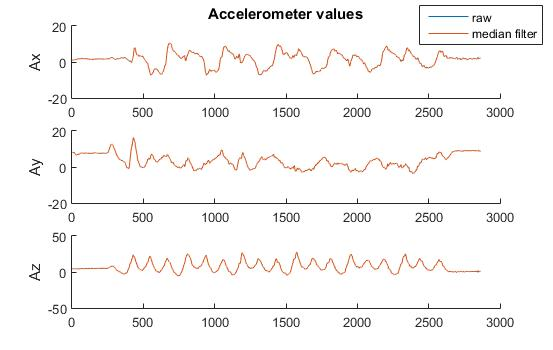
\includegraphics[scale=0.45]{med.jpg}
\caption{Median Filtering}
\label{fig:med}
\end{figure}

The data across all the training sets were clustered using K-means clustering. The inbuilt kmeans matlab function is used for clustering. The maximum number of iterations was set to 500 and the number of clusters were determined from cross validation explained in section \ref{sec:param}. Each 6 dimension datapoint was mapped to the a cluster number to which it belonged. This 1 dimension vector was used as the observation sequence to perform HMM.

\section{Methodology}
\label{sec:hmm}
The implementation follows the method described in \cite{}. The training is implemented using the forward backward and Baum–Welch restimation algorithm. Then the forward algorithm is used to determine the alpha's and hence compute the log likelihood of the the test sequence with respect to each gesture model. 

\subsection{Training}
The forward backward algorithm is used to compute the posterior of all the hidden variables using the given sequence of observations of each training dataset. The number of hidden states N is determined by cross validation. The overview of the algorithm is described below,
\begin{enumerate}
\item The state transition matrices A \& B and initial state $\pi$ were randomly initialized and also normalized. The intial state of hidden variables $\alpha$ and $\beta$ were initialized as,
\begin{align*}
\alpha_1(i) =&\; \pi_i B_i(O_i)), 1\le i \le N \\
\beta_1(i) =&\; 1, 1\le i \le N
\end{align*}
where O is the observation vector obtained from clustering the IMU data using k-means and N is the number of hidden states.
\item alpha is determined for t = 1:T-1 using the induction step.
\begin{align*}
\alpha_{t+1}(j) = \left[\sum_{i=1}^N \alpha_t(i)A_{ij}\right]b_j(O_{t+1})
\end{align*}
At each step alpha is normalized using the sum of all the N elements of $\alpha$ defined as $c_t$. This helps to prevent underflow.
\begin{align*}
c_t = \sum_{i=1}^N \alpha_t(i)
\end{align*}
\item beta is estimated from the end, i.e t = T-1:1 using,
\begin{align*}
\beta_t(i) = \sum_{j=1}^N A_{ij} B_j(O_{t+1}) \beta_{t+1}(j)
\end{align*}
Similar to $\alpha$, $\beta$ is normalized using the sum of all the elements of $\beta$ defined as $d_t$. This helps to prevent underflow.
\begin{align*}
d_t = \sum_{i=1}^N \alpha_t(i)
\end{align*}
\item gamma and Xi are calculated as
\begin{align*}
\gamma(i) =&\; \frac{\alpha_t(i) \beta_t(i)}{\sum_{i=1}^N \alpha_t(i) \beta_t(i)} \\
\xi(i,j) =&\; \frac{\alpha_t(i) A_{ij}B_j(O_{t+1})\beta_{t+1}(j)}{\sum_{i=1}^N \sum_{j=1}^N \alpha_t(i) A_{ij}B_j(O_{t+1})\beta_{t+1}(j)}
\end{align*}
\item Then Baum–Welch restimation equations are used to determine new A, B and Pi using
\begin{align*}
\pi(i) =&\; \gamma(i) \\
A_{ij} =&\; \frac{\sum_{t=1}^{T-1} \xi_t(i,j)}{\sum_{t=1}^{T-1} \gamma_t(i)} \\
B_j(k) =&\;  \frac{\sum_{t=1, s.t.O_t = v_k}^{T} \gamma_t(j)}{\sum_{t=1}^T \gamma_t(j)} \\
\end{align*}
\item This process is repeated unless the log likelihood given by the below equation reaches a threshold
\begin{align*}
log\left[P(O\mid \lambda)\right] =&\; - \sum_{t=1}^T log c_t
\end{align*}
The variation of log likelihood over iterations is shown in Fig. \ref{fig:conv}. It is seen that it converges to a constant value after a few iterations. A threshold of $5 \times 10^{-4}$ could be used to terminate the execution.
\item Two methods were tested for determining the model of each gesture
\begin{itemize}
\item The process described above was repeated for different datasets with random initialization of A, B \& Pi and an average was taken for each gesture.
\item Similar process was followed to determine A,B and Pi for the first dataset of each gesture. Then for the next dataset of the same gesture, the forward backward process was initialized to model parameters A,B and Pi of the first/previous dataset of the same gesture.
\end{itemize}
It was observed that both the models produced a very similar output, but however the latter was less robust as there was a lot of disagreement between beat 3 and beat 4 which have similar motion.
\end{enumerate}

\begin{figure}[hbtp]
\centering
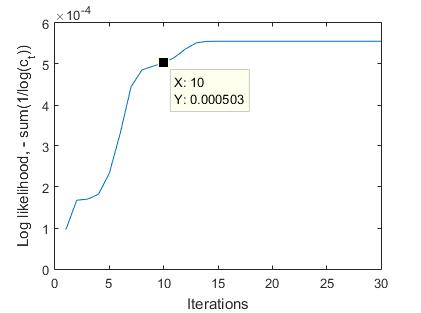
\includegraphics[scale=0.5]{conv.jpg}
\caption{Log liklihood for estimation using Baum–Welch restimation equations}
\label{fig:conv}
\end{figure}

\begin{figure*}
\centering
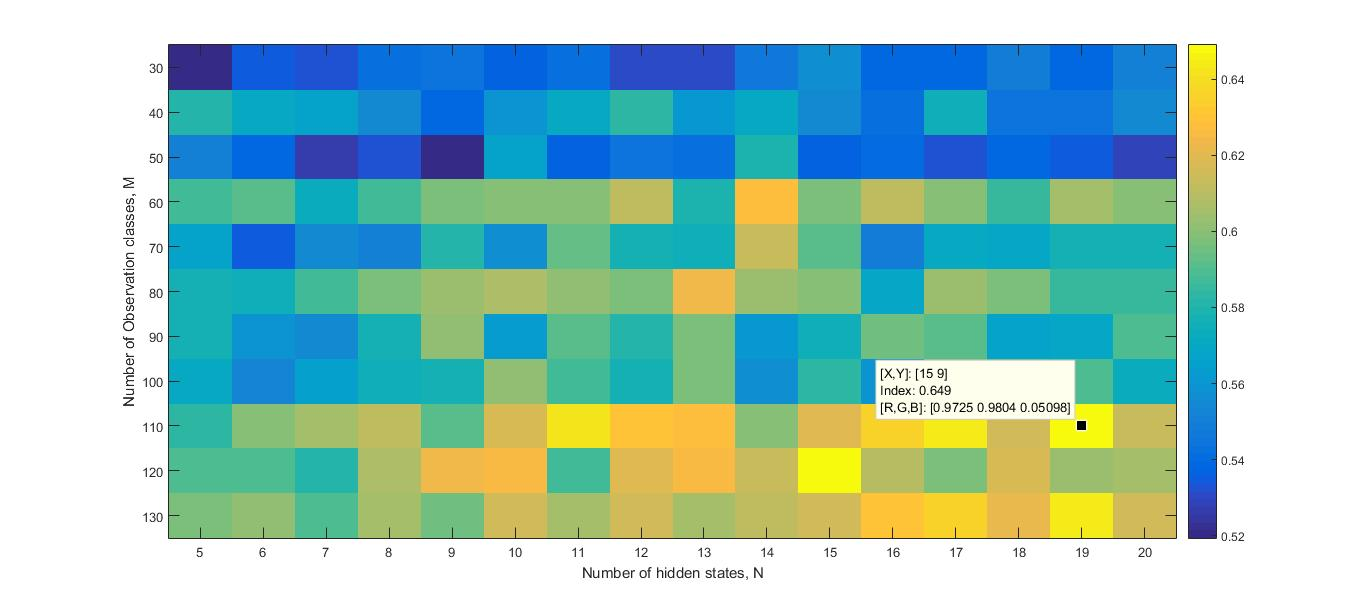
\includegraphics[scale=0.4]{cv.jpg}
\caption{Cross validation results}
\label{fig:cv}
\end{figure*}

\subsection{Testing}
To predict the motion of the new gesture, the log likelihood of the test set with all the trained gesture models was calculated and the gesture with the highest value determined the prediction.
\begin{enumerate}
\item Assign each datapoint of the test set to the respective cluster generated by k-means in section \ref{sec:pprocessing}. This is performed by calculating the minimum distance of the data point to all the cluster centers. This gives us the observation vector O.
\item Determine the hidden state variable $\alpha$ similar to the above training process using the model parameters A, B and Pi for each gesture.
\item Calculate the normalization factor $c_t$ at each time step for each gesture model.
\item Prediction of the system is the model with the highest log likelihood given by,
\begin{align*}
log\left[P(O\mid \lambda)\right] =&\; - \sum_{t=1}^T log c_t
\end{align*}
\vspace{-0.7cm}
\item The confidence was defined as the difference between the first and second log likelihood after normalizing all the likelihood with the maximum value.
\end{enumerate}

\section{Selecting Parameters}
\label{sec:param}
The algorithm uses a number of parameters such as N, number of hidden states and M, number of observation classes. Selecting the right number affects the performance of the system. Hence to determine an optimum value of N and M, cross validation was performed with N ranging from 5 to 20 in steps of 1 and M ranging from 30 to 130 insteps of 10.

 For each pair of N and M LOOCV was performed by randomly choosing 12 train sets as test sets. The median confidence was then used to select the right parameters. Fig. \ref{fig:cv} represents the cross validation results in the form of a color coded matrix, with yellow representing the maximum value. It was seen that the maximum confidence is obtained with N = 19 and M = 110.

Another parameter that affected the performance was how the model parameters was initialized. Two approaches were experimented
\begin{enumerate}
\item A was initialized as a left to right matrix, in which each state could propagate to only 1 other state. B was initialized to a uniform distribution matrix with columns summing to 1. $\pi$ was initialized to first state.
\begin{align*}
A =&\; \begin{bmatrix}
\alpha_1 & 0 & \ldots & 1 - \alpha_N \\
1 - \alpha_1 & \alpha_2 & \ldots & 0 \\
0 & 1 - \alpha_2 & \ldots & 0 \\
\hdots & \hdots & \ddots & \ldots \\
0 & 0 & \ldots & \alpha_N
\end{bmatrix} \\
B =&\; ones(N,M) \times 1/M \\
\pi =&\; [1;0;0;\ldots;0]
\end{align*}
\item Another method used to initialize A, B and $\pi$ is random initialization. There are initialized with a random value and the then normalized across columns such that
\begin{align*}
\sum_{j=1}^N A_{ij} = 1 \quad
\sum_{j=1}^N B_{ij} = 1\quad
\sum_{i=1}^N Pi_{i} = 1 \\
\end{align*}
\end{enumerate}
\vspace{-1cm}
It was seen that the latter method produced more robust results with higher confidence compared to the former. The random initialization was used in this implementation.

\section{Experiments and Results}
\label{sec:results}
The results for various testing sets is tabulated in the Table \ref{tab:res}. The log likelihood graphs are shown in Fig. \ref{fig:test1} to \ref{fig:test8} each for individual test sets. It was seen that most of the test sets were classified correctly with high confidence. But one abnormality that was observed is that the result of test4.txt has a very low confidence and quite often misinterpreted as beat 4 over multiple runs. This is because of the random initialization. It is also affected by the training set chosen to train the model as seen in Fig. \ref{fig:test4err}. 

\begin{table}
\centering
\caption{Predictions for all datasets}
\begin{tabular}{ccccc}
\toprule
Test Set & P1 & P2 & P3 & Confidence \\ 
\midrule
test1.txt & wave & eight & inf & 0.8724 \\
test2.txt & beat 4 & beat 3 & wave & 0.2039 \\ 
test3.txt & inf & eight & beat 3 & 0.7516 \\ 
test4.txt & beat 3 & beat 4 & wave & 0.0316 \\ 
test5.txt & circle & beat 4 & beat 3 & 0.8422 \\ 
test6.txt & inf & eight & beat 3 & 0.7920 \\ 
test7.txt & eight & inf & beat 3 & 0.7592 \\ 
test8.txt & beat 4 & beat 3 & wave & 0.2423 \\ 
\bottomrule
\multicolumn{5}{c}{P1:Prediction 1, P2:Prediction 2 and P3:Prediction 3} \\
\end{tabular} 
\label{tab:res}
\end{table}

\begin{figure}[hbtp]
\centering
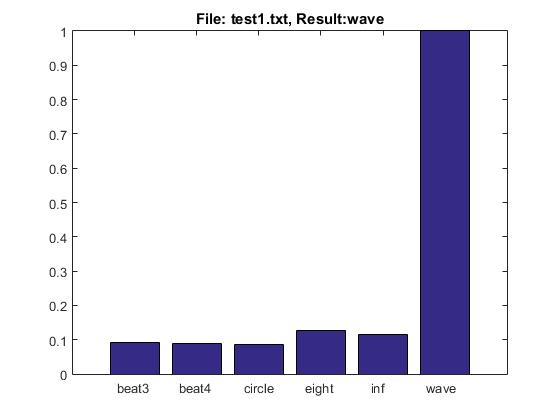
\includegraphics[scale=0.45]{test1.jpg}
\caption{Log likelihood for test1.txt}
\label{fig:test1}
\end{figure}

\begin{figure}[hbtp]
\centering
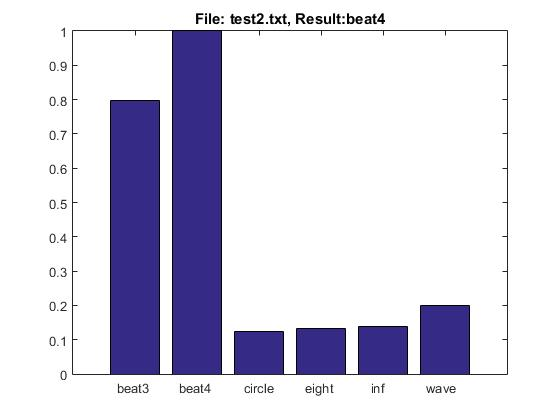
\includegraphics[scale=0.45]{test2.jpg}
\caption{Log likelihood for test2.txt}
\label{fig:test2}
\end{figure}

\begin{figure}[hbtp]
\centering
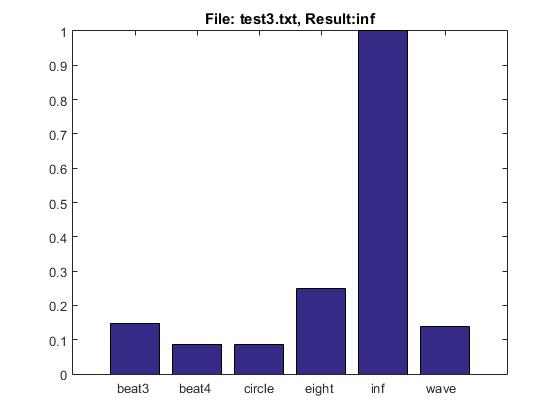
\includegraphics[scale=0.45]{test3.jpg}
\caption{Log likelihood for test3.txt}
\label{fig:test3}
\end{figure}

\begin{figure}[hbtp]
\centering
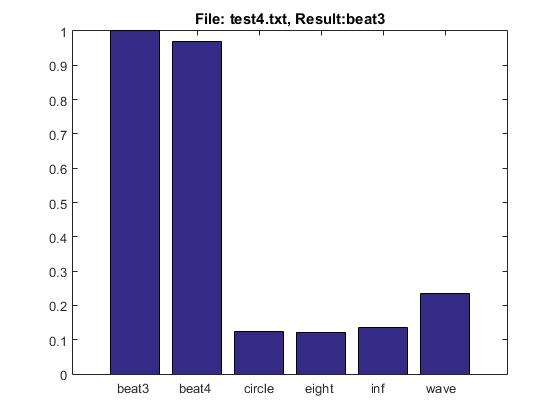
\includegraphics[scale=0.45]{test4.jpg}
\caption{Log likelihood for test4.txt}
\label{fig:test4}
\end{figure}

\begin{figure}[hbtp]
\centering
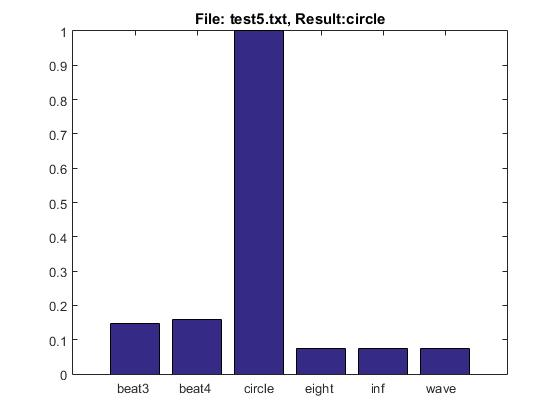
\includegraphics[scale=0.45]{test5.jpg}
\caption{Log likelihood for test5.txt}
\label{fig:test5}
\end{figure}

\begin{figure}[hbtp]
\centering
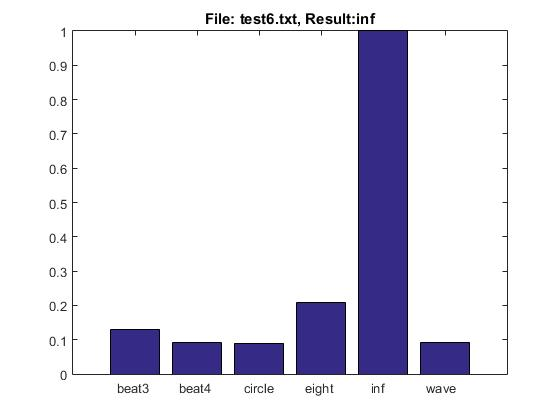
\includegraphics[scale=0.45]{test6.jpg}
\caption{Log likelihood for test6.txt}
\label{fig:test6}
\end{figure}

\begin{figure}[hbtp]
\centering
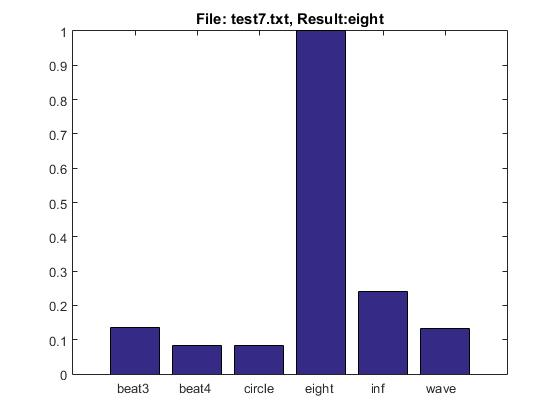
\includegraphics[scale=0.45]{test7.jpg}
\caption{Log likelihood for test7.txt}
\label{fig:test7}
\end{figure}

\begin{figure}[hbtp]
\centering
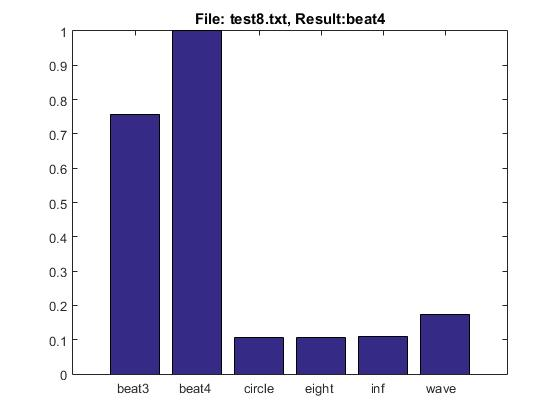
\includegraphics[scale=0.45]{test8.jpg}
\caption{Log likelihood for test8.txt}
\label{fig:test8}
\end{figure}

\begin{figure}[hbtp]
\centering
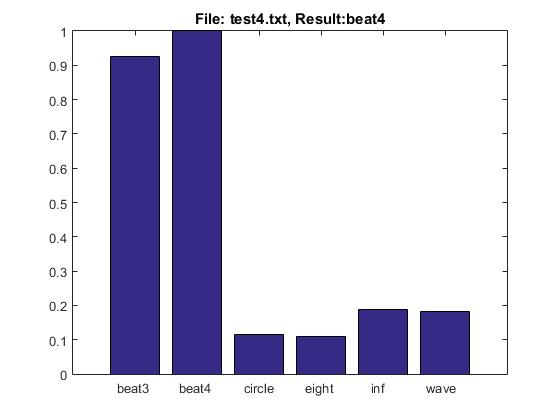
\includegraphics[scale=0.45]{test4err.jpg}
\caption{Log likelihood for test4.txt which was incorrectly classified on few runs}
\label{fig:test4err}
\end{figure}

%\begin{thebibliography}{9}

%\end{thebibliography}

%----------------------------------------------------------------------------------------
%	REFERENCE LIST
%----------------------------------------------------------------------------------------
%\phantomsection
%\bibliographystyle{unsrt}
%\bibliography{sample}

%---------------------------------------------------------------------------------------- 

\end{document}

%% Convergence graph
%% State transition matrixes
%% Cross validation matrix